\documentclass[../../../../document.tex]{subfiles}

\begin{document}
    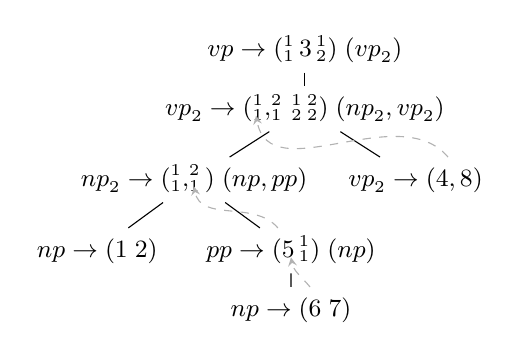
\begin{tikzpicture}[
        level distance=7mm,
        font=\small,
        sibling distance=10mm,
        anchor=center,
        every node/.style={text height=2.5mm},
        rounded corners=0,
        baseline=(mid.base)
        ]

        \begin{scope}[level distance=7.5mm]
            \node (droot) {\(\cn{vp} \to (\x^1_1\,3\,\x^1_2)\;(\cn{vp}_2)\)}
            child {node (tvp) {\(\cn{vp}_2 \to (\x^1_1, \x^2_1\,\x^1_2\,\x^2_2)\;(\cn{np}_2, \cn{vp\binsym}_2)\)}
                [sibling distance=8em, level distance=9mm]
                child {node (mid) {\(\cn{np}_2 \to (\x_1^1, \x^2_1)\;(\cn{np}, \cn{pp})\)}
                    [sibling distance=7em]
                    child {node {\(\cn{np} \to (1\;2)\)}}
                    child {node (pp) {\(\cn{pp} \to (5\,\x^1_1)\;(\cn{np})\)}
                        [level distance=7.5mm]
                        child {node (bnp) {\(\cn{np} \to (6\;7)\)}}}}
                child {node (vpbin) {\(\cn{vp\binsym}_2 \to (4, 8)\)}}};
        \end{scope}


        \begin{scope}[black!30, dashed, >=stealth]
            \draw (vpbin.35) edge[->, out=130, in=-80] (tvp.-155|-tvp.base);
            \draw (bnp.50) edge[->, out=130, in=-80] (pp.-90|-pp.base);
            \draw (pp.120) edge[->, out=130, in=-80] (mid.-90|-mid.base);
        \end{scope}
    \end{tikzpicture}
\end{document}